%! TEX root = 'main.tex'

\section{Background}
\label{sec:ktoctou-background}



\subsection{Kernel-level TOCTOU Vulnerability}

TOCTOU is a type of vulnerability that involves two references on the same variable or system state. The attacker usually passes the first security check with a benign value and then alters it to malicious before the second reference. It is a classic vulnerability, mostly amount file system APIs, which many previous research works have addressed it~\cite{dean2004fixing}~\cite{borisov2005fixing}~\cite{bishop1996checking}~\cite{bishop1995race}~\cite{wei2005tocttou}.


TOCTOU also exists in the operating system kernel. Unlike the classic file system TOCTOU that between APIs, kernel-level TOCTOU appears within individual system calls. When a user program invokes a system call, it usually needs to provide parameters, and it is the kernel's responsibility to verify the legitimacy of the parameters and saves a kernel copy for subsequent use. However, the kernel may fail to accomplish that. Due to the developer's coding style or the unawareness of such vulnerability, the kernel routines do not use the kernel copy; instead, fetch the data from userspace again. Even worse, for historical reasons, a kernel module may not fully decouple with the user-mode components; thus, it directly uses user-mode data.


The double or multiple fetches may lead to a severe issue, as we call it kernel-level TOCTOU vulnerability that attackers usually use to escalate privilege. The parameter sent into the kernel is benign initially to pass the security check; then, the attacker alters it to malicious to introduce an error such as a buffer overflow to the kernel. Although the time window between two kernel fetches may be as narrow as several instructions, it is feasible to create the race condition with careful craft, especially on a multi-processor system.


Due to mistakenly repeated operations on user data, kernel-level TOCTOU widely exists among operating systems~\cite{watson2007exploiting}~\cite{yang2012concurrency}~\cite{lu2008learning}, even in a system such as Linux that use particular gateway functions, \texttt{copy\_to\_user()} and \texttt{copy\_from\_user()}, to get user parameters~\cite{double-fetch-linux}. ~\autoref{table:cves} lists a portion of recent kernel-level TOCTOU vulnerabilities.

\vspace*{-\baselineskip}

\begin{center}
\begin{table}[ht]
%\singlespacing
%\scalebox{0.8}{
\small
\caption{Recent vulnerabilities categorized as race condition or time-of-check-to-time-of-use in the CVE database.}
\label{table:cves}
\centering
	\begin{tabular}{@{}>{\raggedright\arraybackslash}m{2.40cm}@{}|
			@{}>{\centering\arraybackslash}m{1.50cm}@{}|
			@{}>{\centering\arraybackslash}m{2.40cm}@{}|
			@{}>{\centering\arraybackslash}m{1.35cm}@{} } 
\hline
CVE-ID & Affected System & CVE-ID & Affected System \\ %[0.5ex]
\hline
CVE-2008-2252  & Windows & CVE-2016-5728 & Linux \\
CVE-2013-1280  & Windows & CVE-2016-6130 & Linux \\
CVE-2018-7249  & Windows & CVE-2020-9796 & macOS \\ 
CVE-2020-9839  & macOS   & CVE-2020-9990 & macOS \\
CVE-2016-10439 & Android & CVE-2016-7624 & macOS \\
CVE-2016-10383 & Android & CVE-2017-7115 & iOS   \\

CVE-2020-5967  & Nvidia  & CVE-2020-8680 & Intel \\
\hline
\end{tabular}
\end{table}
\end{center}

\vspace*{-\baselineskip}



\begin{figure}[th]
	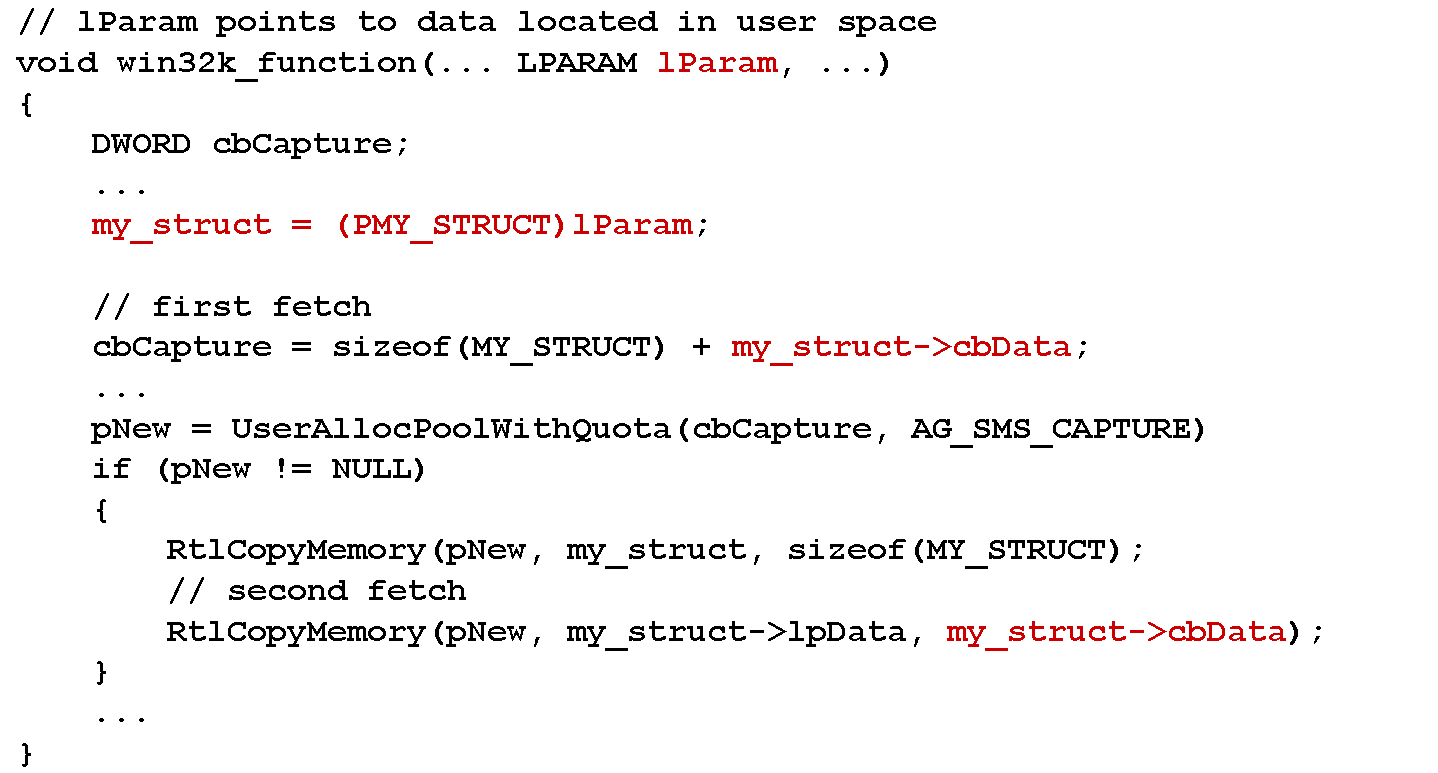
\includegraphics[width=0.47\textwidth]{figures/code08061}
	\centering
	\caption{Pseudocode of the vulnerability fixed in ms08-061. The vulnerable variable is in red. The kernel reads it twice, and it may get a different value for the buffer allocation and the subsequent buffer copying. It is common to see such a coding style. However, it is vulnerable because the two reads cross the privilege boundary.}
	\label{fig:code08061}
\end{figure}



~\autoref{fig:code08061} shows a Windows Win32k module's kernel-level TOCTOU vulnerability~\cite{jurczyk2013identifying}~\cite{ms08061}, which has been identified and patched in Microsoft security bulletins ms08-061. The pseudo-code reassembles to a Win32k system call, and the red part shows the vulnerable data's trace.  The user program passes \texttt{lParam} to \texttt{win32k\_function()} through upper layer APIs.  Adding \texttt{my\_struct->cbData} to \texttt{cbCapture} is where the kernel first gets this user-mode variable and allocates a buffer based on its value. Notice, although there is a local variable called \textit{capture}, the developer forgot to use it subsequently.  Several instructions after, the kernel reread this user-mode variable when copy data into the new buffer.  An attacker can alter the user-mode variable \texttt{my\_struct->cbData} between the two reads, and especially by enlarging it, a kernel buffer overflow is created.


~\autoref{fig:toctouasm} gives the assembly-code-level exploit simulation.  As a local privilege escalation vulnerability, the attacker can invoke the vulnerable system call as many times as needed to succeed. Meantime, thread one is spawned to race with the kernel, aiming to enlarge the user variable. To generate the buffer overflow, the attacker needs to flip the high bit an odd number of times during the time window.


\begin{figure}[ht]
  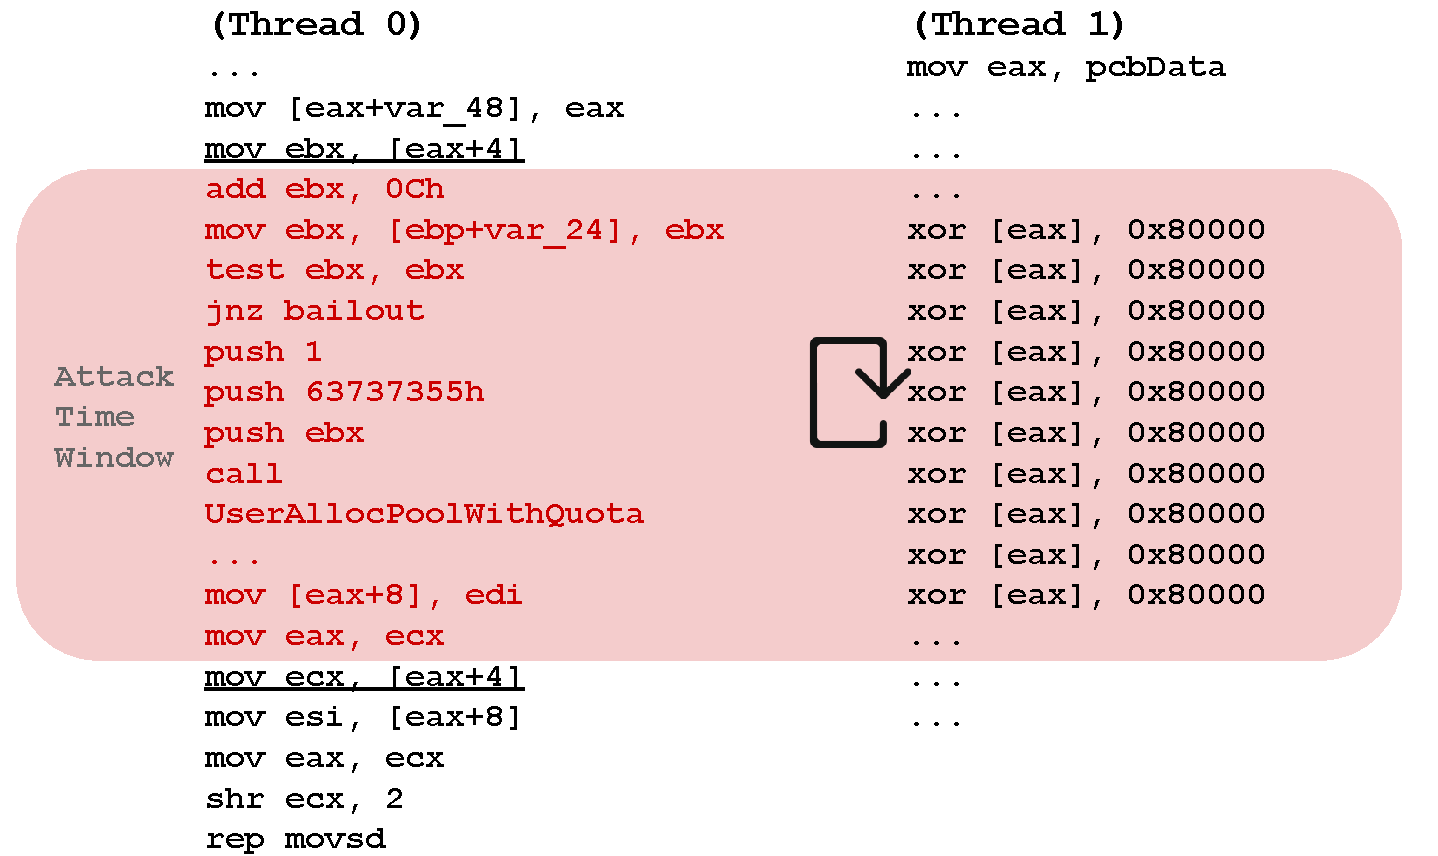
\includegraphics[width=0.47\textwidth]{figures/toctouasm3}
  \centering
  \caption{Thread zero invokes the vulnerable system call. The attack windows lie in between the two kernel reads, namely, the two instructions that underscored. The attacker can repeatedly open the attack time window by calling the system call. Simultaneously, thread one flips the high bit of the user-mode variable in a loop. The two threads compete, hoping an odd number of flips occur during the time window. It enlarges the variable; otherwise, the variable remains the same.}
  \label{fig:toctouasm}
\end{figure}



\subsection{Supervisor Mode Access Prevention (SMAP)}

Monitoring the kernel's userspace behavior is essential to \name. Due to x86 protected mode characteristics, there is no mechanism available for a broad range of monitoring memory modifications. Techniques such as leveraging hardware watchpoints or transactional memory are fittable for fuzzing such vulnerabilities but not for run-time protection. We discuss these two techniques in more details in~\autoref{sec:ktoctou-experiment} and~\autoref{sec:ktoctou-relatedwork}.

Fortunately, we notice an Intel processor feature so-called Supervisor Mode Access Prevention (SMAP)~\cite{corbet2012supervisorsmap} that accurately serves our kernel monitoring requirement.
SMAP is a feature that prevents the kernel from freely accessing userspace so that such access will raise an exception. It complements Supervisor Mode Execution Prevention (SMEP)~\cite{fischer2011supervisor} that introduced earlier. SMEP can be used to prevent the kernel from unintentionally executing user-mode code. SMAP extends this protection to reads and writes. It makes it harder for a malicious program to deceive the kernel into using code or data from the userspace.

Setting SMAP (20) bit in CR4 enables it, and it can also be temporarily disabled by setting the AC flag in EFLAGS or through using \texttt{stac} and \texttt{clac} instructions. Temporarily disabling SMAP usually indicates that the kernel is fully aware of its userspace-access behavior. For example, The Linux kernel supports SMAP since version 3.7. The kernel-to-userspace accesses must go through two gateway functions \texttt{copy\_to\_user()} and \texttt{copy\_from\_user()}, in which SMAP is temporarily disabled.

However, Windows does not support SMAP still. The kernel takes a different approach other than gateway functions; it uses \textit{probe} and \textit{capture} in each system call. \texttt{ProbeForWrite()}  and \texttt{ProbeForRead()}~\cite{probeforread} validates user-mode variables and buffers and this method is effective if done correctly and thoroughly. However, kernel components such as Win32k failed to follow the coding rule.  Some of its code is still coupled with user-mode components. It will cost a huge engineering effort to change the coding style for the enormous codebase.



\subsection{Intel Virtualization Technology}

Intel Virtual-Machine Extensions (VMX) provides hardware-assistant virtualization that adds 13 new instructions: VMPTRLD, VMPTRST, VMCLEAR, VMREAD, VMWRITE, VMCALL, VMLAUNCH, VMRESUME, VMXOFF, VMXON, INVEPT, INVVPID, and VMFUNC. VMX has root and non-root mode, where root mode runs the hypervisor, and the non-root mode runs virtual machines or called guests. On x86 architecture, the processor has four privilege rings. The kernel runs at ring zero, the highest priority ring; the user programs run at ring three; ring one and ring two are unused. With VMX, the root model is commonly viewed as the ring minus one, which is more privileged than ring zero.

VMXON/VMXOFF enters/exits VMX mode. The Virtual Machine Control Structure (VMCS) is the most important data structure, storing the data and states of one virtual processor of one virtual machine. Each core in a physical processor has a VMCS pointer. It points to the physical address of the VMCS. VMPTRLD loads the VMCS pointer from physical memory and set it active and current. VMCLEAR stores VMCS active states back to memory and set it inactive. Although the hypervisor is fully aware of the physical address of each VMCS, it can not modify them directly. All the modifications on VMCS should use the instruction VMREAD and VMWRITE instead.

The VMCS manages aspects of a virtual machine using many data-fields organized into six logical groups: Guest-state area, Host-state area, VM-execution control fields, VM-exit control fields, VM-entry control fields, and VM-exit information fields. The last four groups compose VMX controls that conduct the virtual machine's behavior. In VMX's term, VM entry is the transition from VMX root mode to the non-root mode; VM exit is the opposite. During a VM exit, the processor stores its running state into the Guest-state area in memory and loads the Host-state area into the hardware. The processor does the opposite when entering a virtual machine, the so-called VM entry.



\subsection{x86 Architecture}

In this part, we briefly describe concepts and mechanisms regarding x86 architecture that are used in \name. Some techniques are rarely mentioned in researches but vital to \name. Although IPI and APIC may not technically belong to x86 architecture concepts, we put them here because they are related to the underlying hardware mechanisms.


\textbf{\textit{Paging and Virtual Memory.}} On x86 architecture, with the flat or the segmented memory model, linear address space is mapped into the processors' physical memory space either directly or through paging.  Direct mapping is a one-to-one mapping between the linear address and physical address, also known as the real-mode. When using the paging mode, the linear address space (often referred to as virtual memory) is composed of pages. For simplicity, we only consider 4KB pages in this paper. The pages are backed with physical pages through the Memory Management Unit (MMU), a hardware component that automatically translates virtual addresses to physical addresses using a data structure called the page table. The translation creates the illusion for each process that it has its own large flat virtual memory space (4GB on a 32-bit system).



\textbf{\textit{Page Table.}} The MMU uses page tables to map physical pages to virtual pages~\cite{intelpaging} so that each process in the system can have a flat virtual memory space. Because each process has a page table, the memory used to store those page tables is unignorable. Therefore the system designs a hierarchical data structure to save physical memory. As shown in~\autoref{fig:pagetable}, a virtual address splits into three parts. The last 12-bit is the byte offset of the page;  the first two 10-bit are the index to the page directory and page table. The page tables are also composed of 4KB pages where the system swaps out the long-time unvisited pages to save physical memory. When walking through the page table, we often encounter a swap-out page, which is not an issue because it will be automatically brought back by a page fault regarding page absence. However, this becomes a problem since we are already in the context of a SMAP page fault. The page swap-in process needs the system to read the hard disk, thus more system calls, which inevitably trigger more SMAP exceptions. Eventually, they may cause a dead loop. Therefore, our hypervisor-based solution that confines SMAP at the process level is essential to solving this issue.


\begin{figure}[th]
  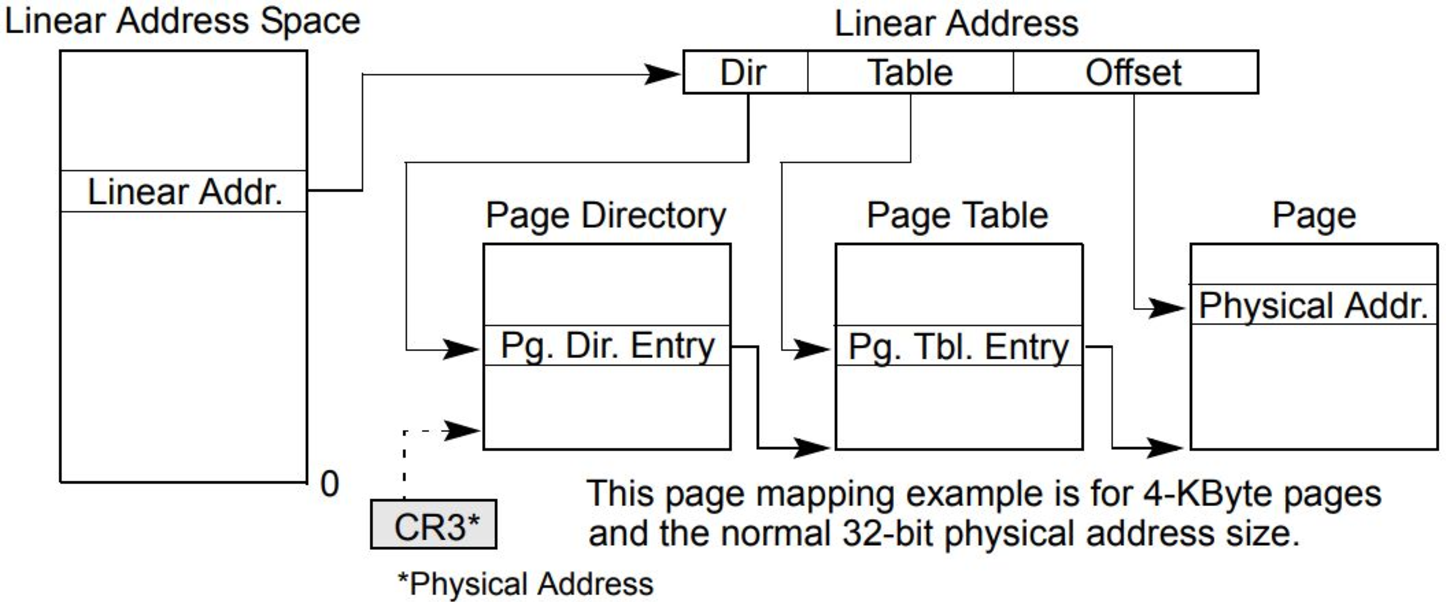
\includegraphics[width=0.47\textwidth]{figures/pagetable}
  \centering
  \caption{Linear-Address Translation to a 4-KBbyte Page using 32-Bit Paging~\cite{intelpaging}}
  \label{fig:pagetable}
\end{figure}



\textbf{\textit{Translation Lookaside Buffer.}} As mentioned above, page table walking is a lengthy process. A full walk needs to access two pages (PD page and PT page). If any of the two pages are not present in the memory, it further triggers a page fault to bring the absent page back.

A Translation Lookaside Buffer (TLB) is part of MMU, and it is a memory cache used to reduce the time to access virtual memory. The TLB has a fixed number of slots that stores the recent translations of virtual memory to physical memory and permission bits. If a valid TLB entry exists, the processor will not walk the page table trying to find the Page Table Entry (PTE). The system kernel is responsible for the consistency between TLB and the page tables.


\textbf{\textit{Interrupt Descriptor Table.}} The Interrupt Descriptor Table (IDT) is a data structure used on the x86 architecture to implement an interrupt vector table. The processor uses the IDT to determine the correct response to interrupts and exceptions.



\textbf{\textit{Interrupt and Exception.}} The fundamental difference in microarchitectural between interrupt and exception is as follows.  An interrupt is an asynchronous event that is typically triggered by an I/O device. An exception is a synchronous event generated when the processor detects one or more predefined conditions while executing an instruction. However, one thing in common is that their handlers are all in the IDT, making them easily confused.

Furthermore, exceptions are categorized as \textbf{faults}, \textbf{traps}, and \textbf{aborts} depending on the way they are raised and whether the instruction that caused the exception can be restarted without loss of program or task continuity. Aborts are not recoverable. They are used to report severe errors, such as hardware errors and inconsistent or illegal values in system tables. Faults and traps are recoverable, and the main difference between them is that when recovers from faults, the return address is the faulting instruction; the trap's return address points to the instruction after the trapping instruction. In our case, the SMAP exception is a fault and handled through the page fault handler.

The IDT has 256 entries. Entry 0-31 are for exceptions, except entry two is for Non-Maskable external Interrupt (NMI). The rest is for external interrupts from INTR pin or \texttt{INT n} instruction. However, \texttt{INT n} also known as a software interrupt. It is essentially an exception with \textit{interrupt} in its name, and its vector located with other external hardware interrupt vectors. Fun.



\textbf{\textit{Trap Frame.}}  The trap frame is a data structure that the processor pushed into the kernel stack when an interrupt or exception occurs. It contains part of the faulting thread's registers. In the context of a page fault, the trap frame contains ErrorCode, CS: EIP, EFLAGS, and SS: ESP. The SS: ESP is included based on whether the CS register's current privacy level (CPL) changes.



\textbf{\textit{Gate.}} Code modules in lower privilege can only access higher privilege modules through a tightly controlled and protected interface called a \textbf{gate}.  There are four types of gate, namely, \textbf{task gate}, \textbf{trap gate}, \textbf{interrupt gate}, and \textbf{call gate}. Fully describe and distinguish them is out of the paper's scope. The project only involves the interrupt gate.

The vectors in the IDT go through either the interrupt gate or trap gate. The difference is subtle. If the interrupt or exception handler is called through an interrupt gate, the processor clears the interrupt flag (IF) in the EFLAGS register to prevent subsequent interrupts from interfering with the handler's execution.  On the other side, when through a trap gate, the processor does not change the IF flag. Setting the interrupt flag is a requirement to control stack depth, which also involves the type of interrupt controller installed in the system. We observed that the processor invokes the page fault handler through an interrupt gate, and we think the reason for that is as follows. The processor loads the CR2 register with the faulting virtual address that caused the exception. If the interruption is allowed in the processor, a thread context switch may swap out the page fault handler, and another page fault occurs subsequently and overwrites the CR2.



\textbf{\textit{CS Segment and Current Privilege Level.}} Unlike other segment registers, the CS segment register cannot be set directly using instruction such as MOV,  but only through a trap or an interrupt gate.  The processor maintains the Current Privilege Level (CPL) field in the CS segment. Thus it is always equal to the processor's current privilege level. The CS register of the trap frame provides us the privilege of the code when the SMAP exception happens. Therefore, we do not make decisions based on EIP's apparent value, making the mitigation more reliable.


\textbf{\textit{Inter-processor Interrupt.}}  It is an interrupt controller mechanism to interrupt another processor or group of processors on the system bus. They are used for software self-interrupts, interrupt forwarding, or preemptive scheduling. In \name, we use IPI to flush the TLB cache on all the processors.


%\textbf{\textit{Local APIC.}} Intel's Advanced Programmable Interrupt Controller (APIC) is a family of interrupt controllers. It is more advanced than Intel's 8259 Programmable Interrupt Controller (PIC). Nowadays, SMP systems with multiple processors utilize APIC. The APIC is a split architecture design, with a local APIC usually integrated into the processor and an optional I/O APIC on a system bus. The local APIC performs two primary functions for the processor:
%It receives interrupts from the processor's interrupt pins, internal sources, and an external I/O APIC. It sends these to the processor core for handling.
%It sends and receives IPI messages to and from other logical processors on the system bus in multiple-processor systems.
%The external I/O APIC is part of Intel's system chipset. It is responsible for receiving interrupts generated by system hardware and I/O devices and forwarding them to the local APIC as interrupt messages. A processor can generate IPIs by programming the interrupt command register (ICR) in its local APIC. Writing to the ICR generates an IPI message on the system bus or the APIC bus. When the target processor receives an IPI message, its local APIC handles the message automatically using information included in the message such as vector number and trigger mode. The IPI mechanism sends interrupts for a specific vector number, and special-purpose interrupts to processors on the system bus. Local APIC registers are memory-mapped to a 4-KByte region of the processor's physical address space with an initial starting address of EFF00000H. The software interacts with the local APIC by reading and writing its registers. It also can change the initial mapping to a different 4-KByte region for all the local APICs. The presence of a local APIC can be detected using the CPUID instruction. Execute CPUID with source operand of 1 in the EAX register, then bit 9 of returned feature flags in EDX register indicate a local APIC.
%
%
%\begin{figure}[th]
%  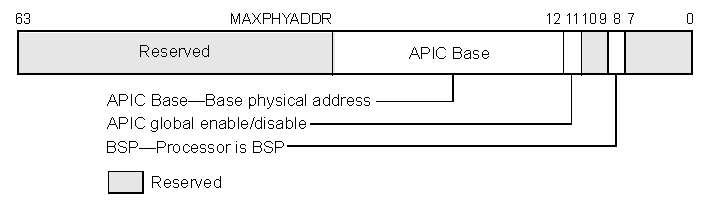
\includegraphics[width=0.47\textwidth]{figures/ia32apicbase}
%  \centering
%  \caption{\texttt{IA32\_APIC\_BASE MSR}}
%  \label{fig:ia32apicbase}
%\end{figure}
%
%There is only one MSR associated with local APIC, \texttt{IA32\_APIC\_BASE}. As shown in~\autoref{fig:ia32apicbase}, the BSP flag indicates if the processor is the bootstrap processor (BSP); ``APIC global enable/disable'' enables/disables the APIC; APIC base specifies the base address of the APIC registers. This 24-bit value needs to be extended by 12 bits at the low end to form the base address. As formerly mentioned, this value by default is 0xFEE00000.
%
%The primary local APIC facility for issuing IPIs is the interrupt command register (ICR), as shown in~\autoref{fig:icr}. It is a 64-bit local APIC register that allows the operating system to specify and send IPIs to processors in the system.
%
%
%\begin{figure}[th]
%  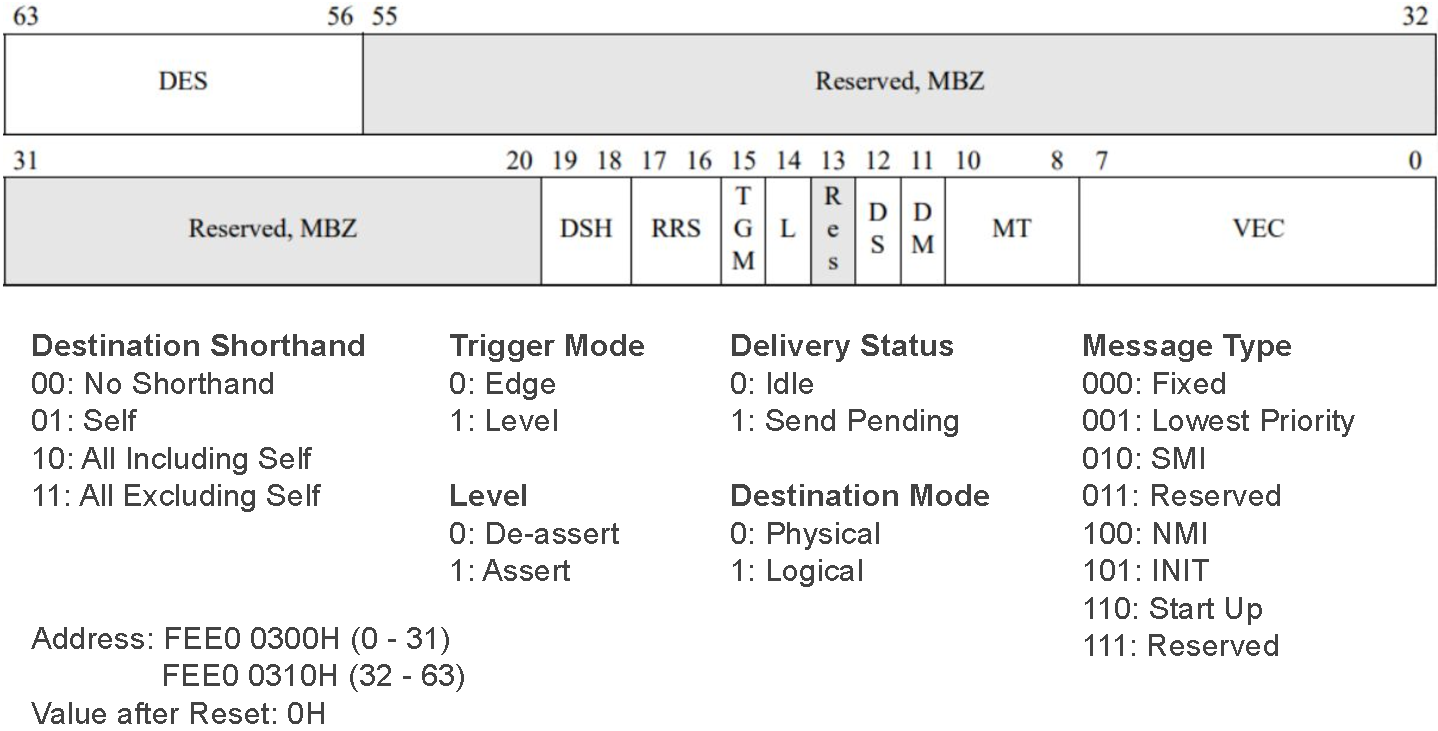
\includegraphics[width=0.47\textwidth]{figures/icr2}
%  \centering
%  \caption{Interrupt Command Register (ICR). Notice, Intel and AMD has slightly different definitions.~\cite{intelapic}~\cite{amdapic}}
%  \label{fig:icr}
%\end{figure}




\textbf{\textit{Inter-processor Interrupt.}}  It is an interrupt controller mechanism to interrupt another processor or group of processors on the system bus. They are used for software self-interrupts, interrupt forwarding, or preemptive scheduling. In \name, we use IPI to flush the TLB cache on all the processors.


\textbf{\textit{Local APIC.}} Intel's Advanced Programmable Interrupt Controller (APIC) is a family of interrupt controllers. Nowadays, multi-processor systems utilize APIC instead of the obsoleted Intel 8259 Programmable Interrupt Controller (PIC). The APIC is a split architecture design, with a local APIC integrated into the processor and the I/O APIC on the system chipset. The local APIC receives interrupts from various sources such as I/O APIC then sends them to the processor, and it also receives/sends IPI messages from/to other processors on the system bus. On the other side, the I/O APIC is responsible for receiving interrupts generated by I/O devices and forwarding them to the local APIC.

A processor can program the local APIC's interrupt command register (ICR) to send out IPIs. The target local APIC receives the IPI message and calls the processor's IDT vector according to the information that comes with it, such as the vector number. Local APIC registers are memory-mapped to a 4-KByte region of the processor's physical address space with an initial starting address at 0xEFF00000. The system software interacts with it through memory operations.


% uty: test  when need to shrink text, the following can go

%\begin{figure}[th]
%  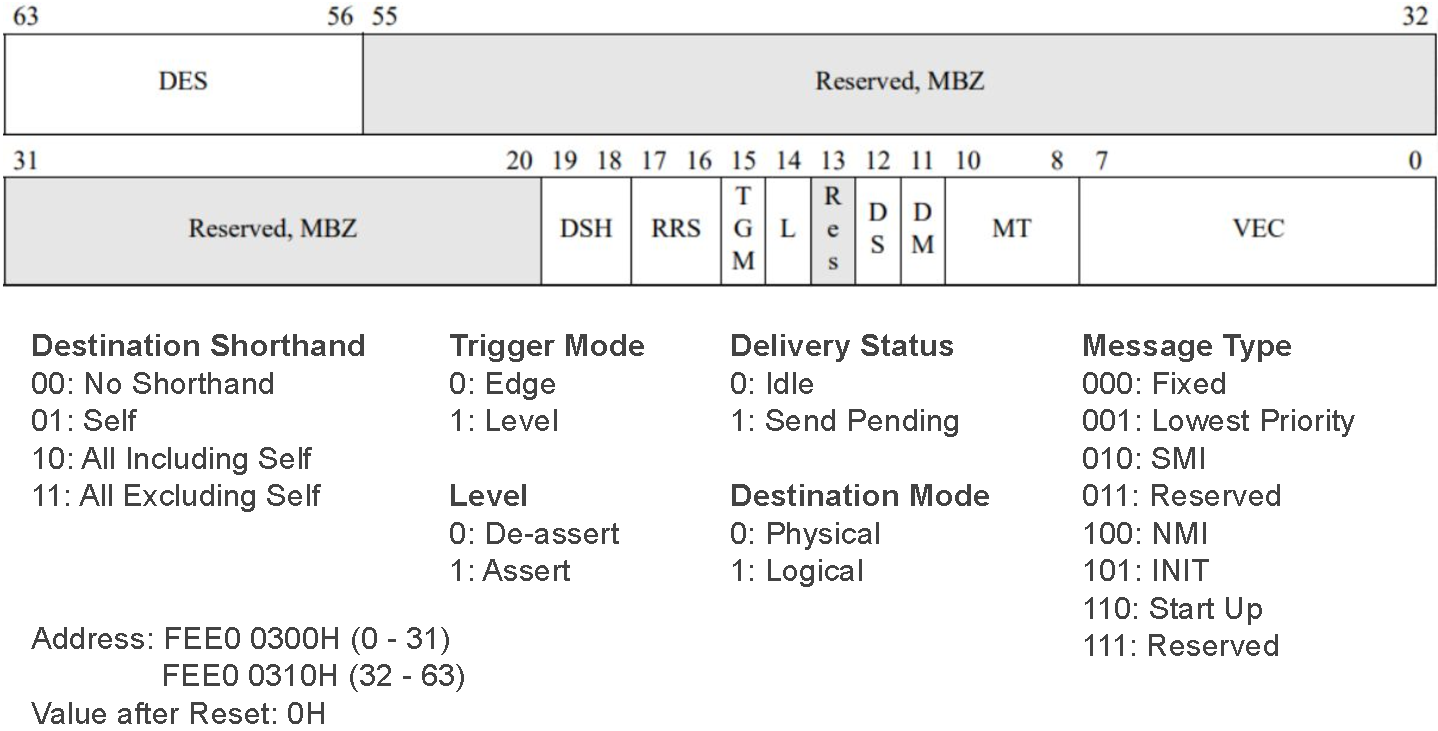
\includegraphics[width=0.47\textwidth]{figures/icr2}
%  \centering
%  \caption{Interrupt Command Register (ICR). Notice, Intel and AMD has slightly different definitions.~\cite{intelapic}~\cite{amdapic}}
%  \label{fig:icr}
%\end{figure}
%
%
%
%~\autoref{fig:icr} shows a 64-bit local APIC register.  In our case, the \textit{Message Type} should be \textit{Fixed} and the \textit{VECTOR} is the IDT slot that we use to handle this IPI.
